\PassOptionsToPackage{unicode=true}{hyperref} % options for packages loaded elsewhere
\PassOptionsToPackage{hyphens}{url}
%
\documentclass[openany]{book}
\usepackage{lmodern}
\usepackage{amssymb,amsmath}
\usepackage{ifxetex,ifluatex}
\usepackage{fixltx2e} % provides \textsubscript
\ifnum 0\ifxetex 1\fi\ifluatex 1\fi=0 % if pdftex
  \usepackage[T1]{fontenc}
  \usepackage[utf8]{inputenc}
  \usepackage{textcomp} % provides euro and other symbols
\else % if luatex or xelatex
  \usepackage{unicode-math}
  \defaultfontfeatures{Ligatures=TeX,Scale=MatchLowercase}
\fi
% use upquote if available, for straight quotes in verbatim environments
\IfFileExists{upquote.sty}{\usepackage{upquote}}{}
% use microtype if available
\IfFileExists{microtype.sty}{%
\usepackage[]{microtype}
\UseMicrotypeSet[protrusion]{basicmath} % disable protrusion for tt fonts
}{}
\IfFileExists{parskip.sty}{%
\usepackage{parskip}
}{% else
\setlength{\parindent}{0pt}
\setlength{\parskip}{6pt plus 2pt minus 1pt}
}
\usepackage{hyperref}
\hypersetup{
            pdftitle={CLU MS Clinical Psychology Thesis Handbook},
            pdfauthor={Jamie Bedics, PhD, ABPP},
            pdfborder={0 0 0},
            breaklinks=true}
\urlstyle{same}  % don't use monospace font for urls
\usepackage{longtable,booktabs}
% Fix footnotes in tables (requires footnote package)
\IfFileExists{footnote.sty}{\usepackage{footnote}\makesavenoteenv{longtable}}{}
\usepackage{graphicx,grffile}
\makeatletter
\def\maxwidth{\ifdim\Gin@nat@width>\linewidth\linewidth\else\Gin@nat@width\fi}
\def\maxheight{\ifdim\Gin@nat@height>\textheight\textheight\else\Gin@nat@height\fi}
\makeatother
% Scale images if necessary, so that they will not overflow the page
% margins by default, and it is still possible to overwrite the defaults
% using explicit options in \includegraphics[width, height, ...]{}
\setkeys{Gin}{width=\maxwidth,height=\maxheight,keepaspectratio}
\setlength{\emergencystretch}{3em}  % prevent overfull lines
\providecommand{\tightlist}{%
  \setlength{\itemsep}{0pt}\setlength{\parskip}{0pt}}
\setcounter{secnumdepth}{5}
% Redefines (sub)paragraphs to behave more like sections
\ifx\paragraph\undefined\else
\let\oldparagraph\paragraph
\renewcommand{\paragraph}[1]{\oldparagraph{#1}\mbox{}}
\fi
\ifx\subparagraph\undefined\else
\let\oldsubparagraph\subparagraph
\renewcommand{\subparagraph}[1]{\oldsubparagraph{#1}\mbox{}}
\fi

% set default figure placement to htbp
\makeatletter
\def\fps@figure{htbp}
\makeatother

\usepackage{booktabs}
\usepackage{amsthm}
\makeatletter
\def\thm@space@setup{%
  \thm@preskip=8pt plus 2pt minus 4pt
  \thm@postskip=\thm@preskip
}
\makeatother
\usepackage[]{natbib}
\bibliographystyle{apalike}

\title{CLU MS Clinical Psychology Thesis Handbook}
\author{Jamie Bedics, PhD, ABPP}
\date{2020-05-12}

\begin{document}
\maketitle

{
\setcounter{tocdepth}{1}
\tableofcontents
}
\hypertarget{goal-of-the-handbook}{%
\chapter{Goal of the Handbook}\label{goal-of-the-handbook}}

\begin{center}\rule{0.5\linewidth}{0.5pt}\end{center}

The goal of this handbook is to provide students with the information needed to successfully complete the master's thesis in the MS in Clinical Psychology Program (MSCP) at California Lutheran University (CLU). The manual should be understood as a supplement to the broader policies and procedures defined by the program and university.

\begin{center}\rule{0.5\linewidth}{0.5pt}\end{center}

\hypertarget{scholarly-research}{%
\section{Scholarly Research}\label{scholarly-research}}

\begin{center}\rule{0.5\linewidth}{0.5pt}\end{center}

Scholarly research requires the skills of inquiry which must be demonstrated by all students. As a participant in research activities at CLU, the University expects you to develop the abilities to:

\begin{enumerate}
\def\labelenumi{\arabic{enumi}.}
\tightlist
\item
  create or contribute empirical knowledge to the existing body of information in a discipline;
\item
  carryout systematic inquiry;
\item
  use tools of research including analyzing existing research, implementing research designs, using and/or developing instrumentation, employing appropriate methods of data analysis, and handling the logistics of conducting a research study;
\item
  work with faculty or other professionals on a research project;
\item
  use scholarly writing techniques.
\end{enumerate}

Research may be a thesis or an independent research project. While both are important contributions to the body of knowledge in a discipline, they have different purposes as described in the following sections.

\begin{center}\rule{0.5\linewidth}{0.5pt}\end{center}

\hypertarget{comprehensive-exam}{%
\section{Comprehensive Exam}\label{comprehensive-exam}}

By default, students entering the MSCP program are required to complete the comprehensive exam. Students can, however, choose to \emph{opt out} of the comprehensive exam and instead complete a thesis.

\textbf{What is the comprehensive exam?}

\begin{itemize}
\tightlist
\item
  A closed book essay test that covers all the material studied during the course
  of the MSCP program.\\
\item
  The test is offered at the end of the spring semester during the second year.
\item
  The exam consists of a morning session (9AM-Noon) and an afternoon session (1PM-4PM).
\item
  During each session, students choose to respond to 3 of 5 questions.
\item
  Instead of credits, students pay a comprehensive exam fee during the semester they
  take the exam.
\item
  Students \emph{do not} have to take PSYC 565, Research Practicum, in the fall and can instead choose an
  additional elective during their second year in the program.
\item
  Students do not take PSYC 566, Thesis, in the spring of their second year.
\end{itemize}

\begin{center}\rule{0.5\linewidth}{0.5pt}\end{center}

\hypertarget{thesis}{%
\section{Thesis}\label{thesis}}

The thesis is the result of an original empirical investigation that creates new knowledge within a discipline. It solves a problem related to lack of knowledge and is generally composed of the following elements:

\begin{enumerate}
\def\labelenumi{\arabic{enumi}.}
\tightlist
\item
  identification of a problem caused by lack of knowledge;
\item
  background and literature review of existing information about the problem;
\item
  methods to be used for obtaining the needed knowledge;
\item
  resulting new knowledge;
\item
  interpretation of the new knowledge.
\item
  transparent and open sharing of materials and results via pre-registration and the open science framework
\end{enumerate}

\textbf{Tasks:}

\begin{itemize}
\tightlist
\item
  Students complete all the requirements outline in this manual
\item
  Students enroll in PSYC 565, Research Practicum, during the fall of their second year
\item
  Students enroll in PSYC 566, Thesis, during the spring of their second year
\end{itemize}

\begin{center}\rule{0.5\linewidth}{0.5pt}\end{center}

\hypertarget{pros-and-cons-thesis-vs.-comps}{%
\section{Pros and Cons: Thesis Vs. Comps}\label{pros-and-cons-thesis-vs.-comps}}

\emph{Thesis ``Pros''}

\begin{itemize}
\tightlist
\item
  Students gain a high degree of expertise and mastery in the particular area under study.
\item
  The thesis timeline creates accountability and structure in developing students' research project.
\item
  Doctoral programs might look favorably towards a completed thesis that demonstrates students ability to complete an independent research project.
\item
  Doctoral programs that require a thesis might waive the thesis requirement based on students' completed thesis at CLU.
\item
  Students can have the thesis bound into a book.
\end{itemize}

\emph{Thesis ``Cons''}

\begin{itemize}
\tightlist
\item
  Despite the structure offered through coursework, the thesis requires a considerable amount of work and self-discipline and the stress associate with this extra work.
\item
  Students take an extra 3-units (PSYC 566) in the spring of their second year for a total of 40-units versus 37-units for the comprehensive exam option.
\end{itemize}

\begin{center}\rule{0.5\linewidth}{0.5pt}\end{center}

\emph{Comps ``Pros''}

\begin{itemize}
\tightlist
\item
  A review sheet is provided to help focus student's efforts to study.
\item
  The exam is done in a day.
\item
  Questions that are not adequately answered can be remitted before ``failing.''
\item
  The pressure to meet thesis requirements, every semester, is removed.
\item
  Students can still complete an \textbf{research project} (see next section) which would allow the first three \emph{thesis pros} to be achieved.
\item
  Students choose a 3-credit elective during their second year.
\item
  The entire program is 37-units versus 40-units with the thesis option.
\end{itemize}

\emph{Comps ``Cons''}

\begin{itemize}
\tightlist
\item
  A 6-hour, closed book, essay test can be stressful and exhausting.
\item
  The research project could not be as structured as the thesis option.
\end{itemize}

\begin{center}\rule{0.5\linewidth}{0.5pt}\end{center}

\hypertarget{research-project-option}{%
\section{Research Project Option}\label{research-project-option}}

\textbf{Research Project + Comprehensive Exam}

Students can complete their own independent research project, identical to the thesis, but without the coursework (PSYC 565 \& PSCY 566). There are two scenarios where this can occur:

\begin{enumerate}
\def\labelenumi{\arabic{enumi}.}
\tightlist
\item
  A student can decide, from the beginning of the program, that they want to avoid the pressure and extra work of the thesis requirements but use the program to work on an research project. They could take PSYC 565 in the fall of their second year but will not take PSYC 566 during the spring.
\item
  Students might attempt the thesis but, for a variety of reasons, fall behind and be removed from or quite the thesis track.
\end{enumerate}

In both of these scenarios, students are required to take the comprehensive exam and pay the comprehensive exam fee, in order to graduate. The student can, however, continue to work on their independent research project but not for credit.

\begin{center}\rule{0.5\linewidth}{0.5pt}\end{center}

\hypertarget{thesis-checklist}{%
\chapter{Thesis Checklist}\label{thesis-checklist}}

Students who wish to pursue the thesis option are required to meet with Dr.~Bedics at the end of every semester in order to review their progress according to the following timeline.
Students who miss any of the following steps are removed from the thesis option and will be required to complete the comprehensive exam.

\begin{longtable}[]{@{}lllll@{}}
\toprule
& Task & Date Due & Year & Finished\tabularnewline
\midrule
\endhead
1. & Thesis Topic Approved & October 1st & First Year & {[}\_\_\_\_\_{]}\tabularnewline
2. & Setup OSF & October 1st & First Year & {[}\_\_\_\_\_{]}\tabularnewline
3. & Literature Review Draft Psych 564 & December 15th & First Year & {[}\_\_\_\_\_{]}\tabularnewline
4. & Academic Good Standing & December 15th & First Year & {[}\_\_\_\_\_{]}\tabularnewline
5. & Method Section Draft & May 1st & First Year & {[}\_\_\_\_\_{]}\tabularnewline
6. & Literature Review Revision & May 1st & First Year & {[}\_\_\_\_\_{]}\tabularnewline
7. & Academic Good Standing & May 15th & First Year & {[}\_\_\_\_\_{]}\tabularnewline
8. & Committee Assignment & June 30th & Summer & {[}\_\_{]} Chair{[}\_\_{]} Reader\tabularnewline
9. & Academic Good Standing & July 3rd & Summer & {[}\_\_\_\_\_{]}\tabularnewline
10. & Enroll in PSYC 565 & August 1st & Second Year & {[}\_\_\_\_\_{]}\tabularnewline
11. & Committee Approval of Proposal & October 1st & Second Year & {[}\_\_\_\_\_{]}\tabularnewline
12. & IRB Submitted & November 1st & Second Year & {[}\_\_\_\_\_{]}\tabularnewline
13. & Academic Good Standing & December 15th & Second Year & {[}\_\_\_\_\_{]}\tabularnewline
14. & Enroll in PSYC 566 & December 15th & Second Year & {[}\_\_\_\_\_{]}\tabularnewline
15. & Complete Draft to Dr.~Bedics & May 1st & Second Year & {[}\_\_\_\_\_{]}\tabularnewline
16. & Committee Approval of Final & May 10th & Second Year & {[}\_\_{]} Chair{[}\_\_{]} Reader\tabularnewline
17. & OSF Approval & May 1st & Second Year & {[}\_\_\_\_\_{]}\tabularnewline
18. & Thesis Commons & May 15th & Second Year & {[}\_\_\_\_\_{]}\tabularnewline
19. & Thesis Binding & Optional & Second Year & {[}\_\_\_\_\_{]}\tabularnewline
20. & GitHub Blog & Optional & Second Year & {[}\_\_\_\_\_{]}\tabularnewline
21. & Shiny App & Optional & Second Year & {[}\_\_\_\_\_{]}\tabularnewline
\bottomrule
\end{longtable}

\hypertarget{thesis-topic}{%
\section{Thesis Topic}\label{thesis-topic}}

\begin{center}\rule{0.5\linewidth}{0.5pt}\end{center}

\textbf{Defining the Problem Area}

The general thesis topic is required to be selected during the beginning of the first semester of the first year. The thesis topic, does not, however, determine the hypotheses, methodology or general approach taken by the student to understand the problem (e.g.~experimental, quasi-experimental, meta-analytic methods). It would be premature for a student to define a hypothesis in the first year when their understanding of the topic area is just beginning. Hypotheses are typically developed after the first year of study.

\textbf{Due}: October 1st, First Year

\begin{center}\rule{0.5\linewidth}{0.5pt}\end{center}

\hypertarget{open-science-framework}{%
\section{Open Science Framework}\label{open-science-framework}}

\textbf{Creating a transparent and reproducible workflow}

\href{https://osf.io/}{OSF} is repository that allows you to transparenlty share your work with the larger scientific community. During the course of the program, you will be using the OSF to organize your thesis and other independent research projects. Instructions for setting up an OSF project can be found \href{https://speakerdeck.com/jdbedics/osf-setup-and-class-project-introduction}{here} and will be reviewed with Dr.~Bedics at your first advising meeting.

\textbf{Due}: October 1st, First Year

\begin{center}\rule{0.5\linewidth}{0.5pt}\end{center}

\hypertarget{literature-review}{%
\section{Literature Review}\label{literature-review}}

\begin{center}\rule{0.5\linewidth}{0.5pt}\end{center}

\textbf{Understanding the Problem}

The development of the literature review begins during the fall of the first year during PSYC 564 Advanced Research Methods. The literature review will become the ``introduction'' section of the final thesis paper. The literature review demonstrates the student's mastery of the literature surrounding the \emph{problem} to be addressed by the thesis.

Initial drafts, such as that from PSYC 564, are 10-12 pages in length. The development of the literature review is, however, ongoing throughout the two years of the program until the final draft is submitted on May 1st of the second year.

The typical length of a \emph{complete} literature review is between \textbf{20-40 pages} long but there is no maximum length.

\textbf{Due}: December 15th, First year (First Major Draft); May 15th, end of first year (Second Major Draft); May 1st, end of second year (Final Draft)

\begin{center}\rule{0.5\linewidth}{0.5pt}\end{center}

\hypertarget{method-section}{%
\section{Method Section}\label{method-section}}

\begin{center}\rule{0.5\linewidth}{0.5pt}\end{center}

\textbf{Solving the Problem}

The method sections defines the procedures of the thesis. The method section consists of the participant selection, selection of methods of measurements or materials, and the procedure. The method section can be worked on in PSYC 552 Psychometrics during spring of the first year and is finalized during PSYC 565 in the fall of the second year.

\textbf{Due}: May 1st, First Year (First Draft)

\begin{center}\rule{0.5\linewidth}{0.5pt}\end{center}

\hypertarget{committee-assignment}{%
\section{Committee Assignment}\label{committee-assignment}}

\begin{center}\rule{0.5\linewidth}{0.5pt}\end{center}

Committee members are faculty or experts in the field that support the students work on the thesis. Students work with the program director to find the most appropriate committee members to support their research project. See the Committee section of this handbook.

\textbf{Due}: June 30th, Summer after First Year

\begin{center}\rule{0.5\linewidth}{0.5pt}\end{center}

\hypertarget{committee-approval-of-proposal}{%
\section{Committee Approval of Proposal}\label{committee-approval-of-proposal}}

\begin{center}\rule{0.5\linewidth}{0.5pt}\end{center}

During the summer following the first year, committee members read the literature review and method section and provide a general statement of approval to Dr.~Bedics. Based upon this approval, students are allowed to progress to the \emph{thesis track.} The rest of the thesis process is guided through coursework including PSYC 565 Research Practicum in the fall of the second year and PSYC 566 Thesis in the spring of the second year.

\textbf{Due}: October 1st, Second Year

\begin{center}\rule{0.5\linewidth}{0.5pt}\end{center}

\hypertarget{academic-good-standing}{%
\section{Academic Good Standing}\label{academic-good-standing}}

\begin{center}\rule{0.5\linewidth}{0.5pt}\end{center}

Academic good standing refers to maintaining a GPA above a 3.0 throughout the entire program and acting consistently with all policies and procedures defined by the program (see Program Handbook) and university (see university policy and procedures). Any student who receives below a B- in any course is not allowed to complete the thesis for course credit and partial fulfillment of the degree.

\textbf{Due}: Every semester

\begin{center}\rule{0.5\linewidth}{0.5pt}\end{center}

\hypertarget{coursework-relevant-to-the-thesis}{%
\chapter{Coursework Relevant to the Thesis}\label{coursework-relevant-to-the-thesis}}

\begin{center}\rule{0.5\linewidth}{0.5pt}\end{center}

The knowledge gained from each course taken can be used to improve the development of the thesis. For example, if you have a particular interest in a specific disorder then it makes sense that you study that disorder in \emph{PSYC 510 Psychopathology}. In \emph{PSYC 560 Statistics I: Exploratory Data Analysis}, you might consider finding open data that allows you to better understand your problem area through data visualization. For example, if a student was interested in suicide they could examine open data from WHO and examine changing incidence rates across time and by countries.

There are, however, specific courses where the thesis is explicitly incorporated into assignments. The following are the MSCP courses that explicitly incorporate elements of the thesis into the syllabi:

\begin{longtable}[]{@{}lllll@{}}
\toprule
PSYC\# & Course & Semester & Year & Task\tabularnewline
\midrule
\endhead
564 & Adv. Research Methods & Fall & One & Literature Review\tabularnewline
562 & Statistics II: Regression & Spring & One & Data Analytic Plan\tabularnewline
552 & Psychometrics & Spring & One & Method\tabularnewline
521 & Ethics & Summer & One & Pre-Registration\tabularnewline
565 & Research Practicum & Fall & Two & IRB, Intro, Method\tabularnewline
566 & Thesis & Spring & Two & Complete Draft due May 1st\tabularnewline
\bottomrule
\end{longtable}

\hypertarget{formatting}{%
\chapter{Formatting}\label{formatting}}

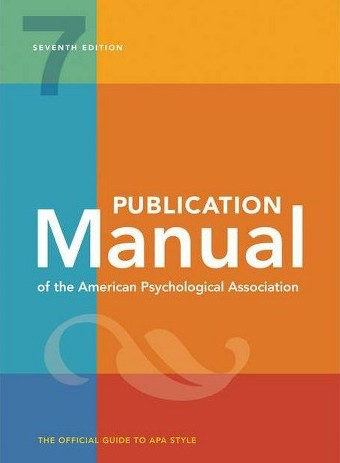
\includegraphics[width=4.72in]{images/apamanual}

The thesis paper is completed in a manner consistent with the \href{https://www.amazon.com/s?k=apa+publication+manual+7th+edition\&crid=7T10VJ2PYQZH\&sprefix=apa+pu\%2Caps\%2C261\&ref=nb_sb_ss_i_1_6}{Publication Manual of the APA (7th Edition)}. Specifically, the following sections should follow, exactly, the guidelines defined by the 7th Edition:

\begin{itemize}
\tightlist
\item
  Abstract
\item
  Introduction
\item
  Method
\item
  Results
\item
  Discussion
\item
  References
\item
  Tables
\item
  Figures
\item
  Appendices
\end{itemize}

There are several sections that \textbf{do not} follow the 7th Edition of the Publication Manual:

\begin{itemize}
\tightlist
\item
  Title Page
\item
  Table of Contents
\end{itemize}

For examples of these, please see the Thesis Materials section of the MSCP homepage in Blackboard. General guidelines can be followed below:

\begin{center}\rule{0.5\linewidth}{0.5pt}\end{center}

\hypertarget{title-page-guidelines}{%
\section{Title Page Guidelines}\label{title-page-guidelines}}

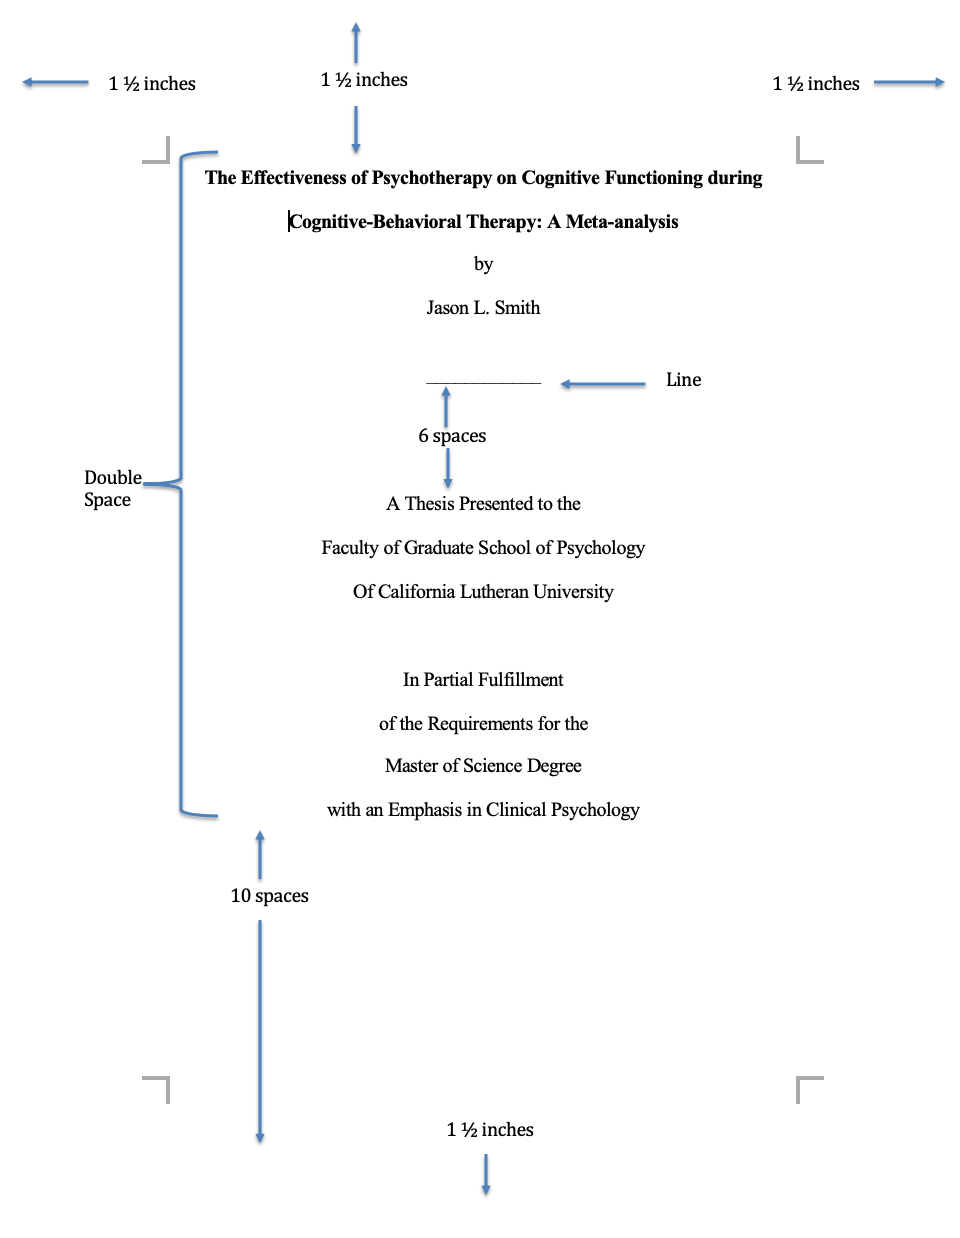
\includegraphics[width=13.33in]{images/titlepage}

\hypertarget{signature-page-guidelines}{%
\section{Signature Page Guidelines}\label{signature-page-guidelines}}

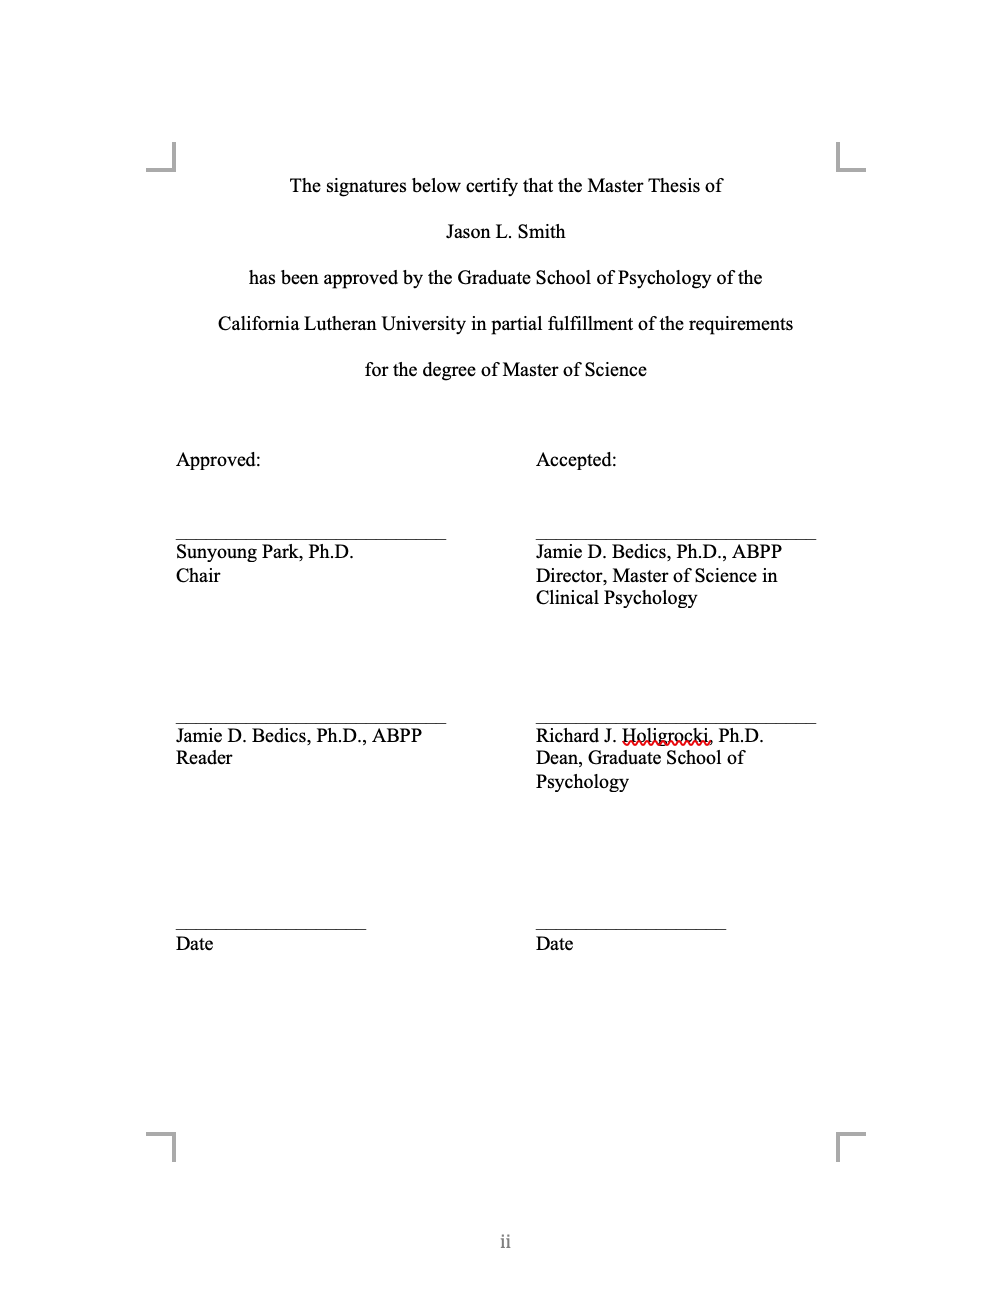
\includegraphics[width=13.94in]{images/signaturepage}

\hypertarget{table-of-contents-guidelines}{%
\section{Table of Contents Guidelines}\label{table-of-contents-guidelines}}

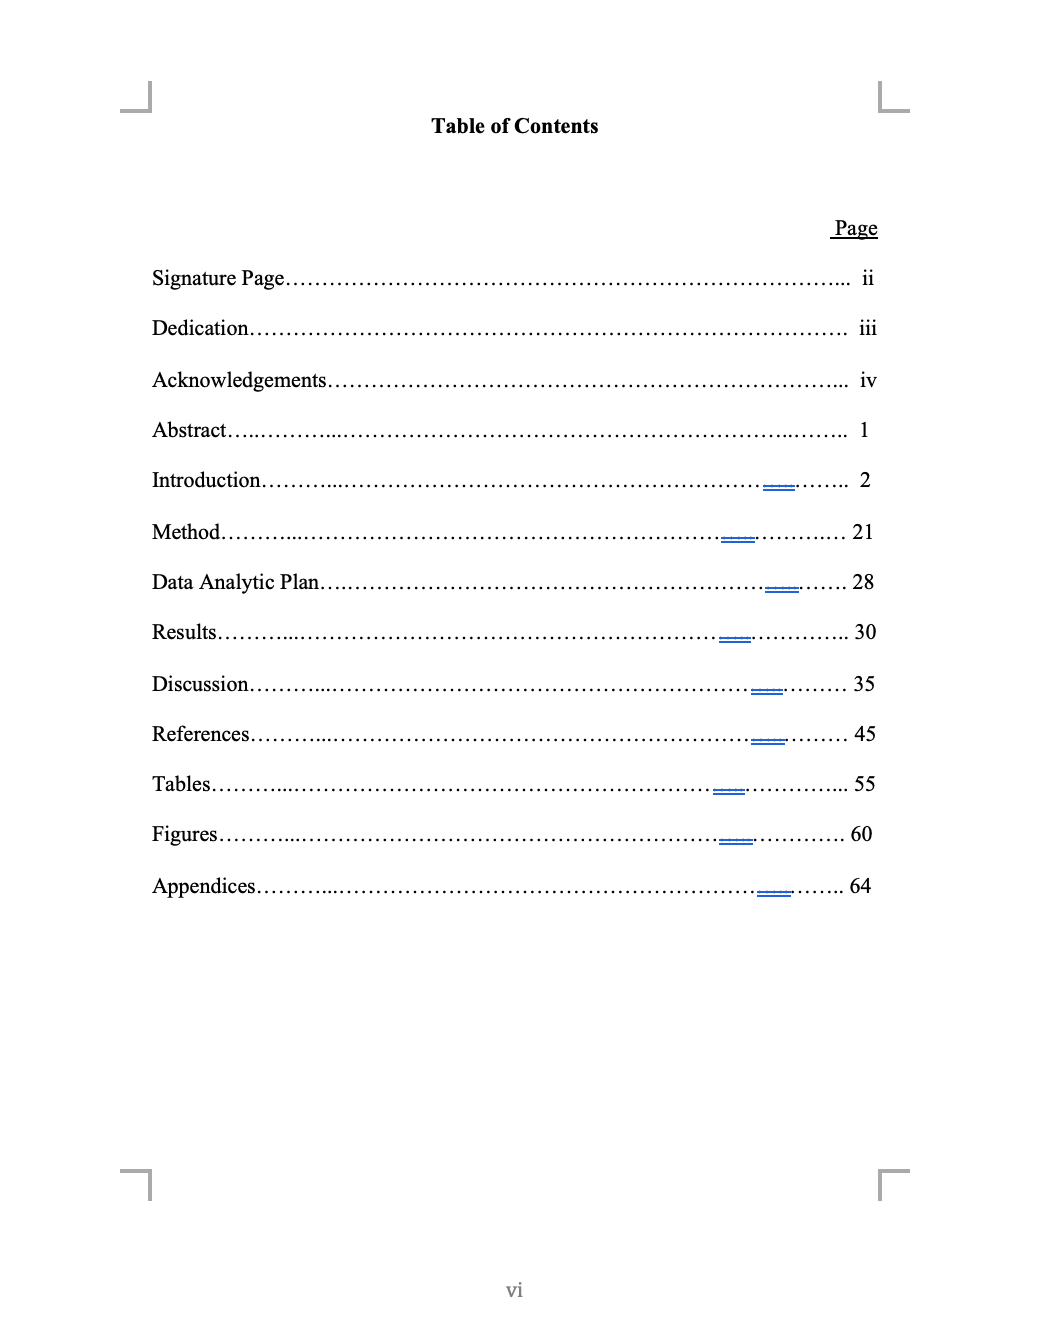
\includegraphics[width=14.58in]{images/tablecontents}

\hypertarget{final-ordering}{%
\section{Final Ordering}\label{final-ordering}}

\textbf{1. Title Page (according to CLU format and not APA)}

This page provides the name of the thesis project, names of the university and school or department, and date of completion. The title page should be prepared in accordance with the sample page found in this section. The date at the bottom of the page is the month and year the degree is awarded. The title page is unnumbered but is counted as page ``i.''

\begin{center}\rule{0.5\linewidth}{0.5pt}\end{center}

\textbf{2. Signature Page (according to CLU format and not APA)}

This page provides the name of the author and blank lines for the signatures of the committee members and the Graduate Dean of the appropriate School. The pages are signed when the members and Dean determine that the thesis or project is complete. The approval page should comply with the page form found in Appendix B. It should bear original signatures for all copies. The date at the bottom of the page is the date the degree is awarded; however, the page is not counted in the numbering system.

\begin{center}\rule{0.5\linewidth}{0.5pt}\end{center}

\textbf{3. Dedication (optional)}

This optional page contains a brief dedication to the individual(s) whom the author wishes to honor. If included, thispageisnumberedaspage``ii'' (lowercaseRomannumeral).

\begin{center}\rule{0.5\linewidth}{0.5pt}\end{center}

\textbf{4. Acknowledgements (optional)}

This optional page lists persons and/ or institutions whom the author wishes to thank for their assistance in completing the thesis or project. Such assistance can be provision of personal, financial, or moral support, or access to data sets or subject populations. A brief statement as to the type of assistance provided may follow each person or institution named. If included, this page continues the lower case R oman numeral sequence begun above.

\begin{center}\rule{0.5\linewidth}{0.5pt}\end{center}

\textbf{5. Table of Contencts (accoridng to CLU format)}

\begin{center}\rule{0.5\linewidth}{0.5pt}\end{center}

\textbf{6. Abstract (APA style)}

\begin{center}\rule{0.5\linewidth}{0.5pt}\end{center}

\textbf{7. Introduction (APA style)}

\begin{center}\rule{0.5\linewidth}{0.5pt}\end{center}

\textbf{8. Method (APA style)}

\begin{center}\rule{0.5\linewidth}{0.5pt}\end{center}

\textbf{9. Data Analytic Method (APA style)}

\begin{center}\rule{0.5\linewidth}{0.5pt}\end{center}

\textbf{10. Results (APA style)}

\begin{center}\rule{0.5\linewidth}{0.5pt}\end{center}

\textbf{11. Discussion (APA style)}

\begin{center}\rule{0.5\linewidth}{0.5pt}\end{center}

\textbf{12. References (APA style)}

\begin{center}\rule{0.5\linewidth}{0.5pt}\end{center}

\textbf{13. Tables (APA style)}

\begin{center}\rule{0.5\linewidth}{0.5pt}\end{center}

\textbf{14. Figures (APA style)}

\begin{center}\rule{0.5\linewidth}{0.5pt}\end{center}

\textbf{15. Appendix 1 - Pre-Registration}

\begin{center}\rule{0.5\linewidth}{0.5pt}\end{center}

\textbf{16. Appendix 2 - IRB Approval}

\begin{center}\rule{0.5\linewidth}{0.5pt}\end{center}

\textbf{17. Appendix \# - optional as needed}

\begin{center}\rule{0.5\linewidth}{0.5pt}\end{center}

\hypertarget{thesis-binding}{%
\chapter{Thesis Binding}\label{thesis-binding}}

The following are instructions for binding your thesis. The binding of your thesis is \emph{optional} and at your expense.You are responsible for the spelling, grammar, and correct APA formatting of your thesis. A bound thesis is a \textbf{final} thesis.

\begin{enumerate}
\def\labelenumi{\arabic{enumi}.}
\tightlist
\item
  At least three (3) bound copies of the Thesis must be ordered.

  \begin{enumerate}
  \def\labelenumii{\alph{enumii}.}
  \tightlist
  \item
    One copy for the Graduate School of Psychology, one copy for the Thesis Committee Chair, and one personal copy for your possession. You can order more if you prefer (see \#2).
  \item
    The three copies must be printed on 25\% rag or cotton fiber watermarked white paper, at least 20 pound weight, 8½ x 11 inches in size (EZERASE, or similar paper is not acceptable). A good example is Southworth Fine Business Paper, 25\% cotton, 24 pound, white, stock \#403C which is available for purchase from Office Depot, OfficeMax, and Staples. A similar 20 pound weight paper is also available.
  \item
    Original signed signature pages on the same paper must be submitted with each of the three copies.
  \end{enumerate}
\item
  Additional personal copies may be ordered at the same time.

  \begin{enumerate}
  \def\labelenumii{\alph{enumii}.}
  \tightlist
  \item
    Personal copies may be printed on paper of the student's choice (e.g., 20 pound paper).
  \item
    Signature pages for the personal copies may be photocopies of the originals as long as they are on paper that is identical to the rest of the thesis.
  \end{enumerate}
\item
  Copies for binding must be delivered to the Program Specialist.

  \begin{enumerate}
  \def\labelenumii{\alph{enumii}.}
  \tightlist
  \item
    The copies delivered to the Program Specialist are NOT to be bound - just packaged with bright colored paper separating the individual copies.
  \item
    Students are responsible for paying binding fees for all copies (the three required copies and for any additional personal copies). The cost is \$40 per copy (no matter the length), and to be paid by check to CLU. Prices may change.
  \item
    The Program Specialist will forward the copies to the bindery as they are delivered.
  \item
    Once the Program Specialist receives the copies and payment for binding, a change of grade will be submitted to the Registrar's Office.
  \end{enumerate}
\item
  The bound copies are typically ready in about 6-8 weeks and are distributed as follows:

  \begin{enumerate}
  \def\labelenumii{\alph{enumii}.}
  \tightlist
  \item
    The Graduate School of Psychology copy and the Thesis Committee Chair copy will be delivered via campus mail by the Program Specialist.
  \item
    Students will be notified when their personal copies are ready for pick-up.
  \end{enumerate}
\item
  If you have any questions regarding the binding process, please do not hesitate to contact Mengmeng Liu, Graduate Program Specialist, at 805-493-3662 or at \href{mailto:mengmengliu@callutheran.edu}{\nolinkurl{mengmengliu@callutheran.edu}}.
\end{enumerate}

\hypertarget{thesis-commons}{%
\chapter{Thesis Commons}\label{thesis-commons}}

\href{https://thesiscommons.org/}{Thesis Commons} is a place for you publish your thesis to be seen by others. Thesis Commons is supported by OSF and is a way to both archive and showcase your work along with your OSF project.

\hypertarget{presentations-and-publications}{%
\chapter{Presentations and Publications}\label{presentations-and-publications}}

The faculty hope you present your work at conferences and in publications. Please remember to contact your chair \emph{prior} to submitting your work to any professional outlet. Your committee will typically be authors on all of your publically published work.

\bibliography{book.bib,packages.bib}

\end{document}
